% !TEX program = xelatex
% 第一讲：生成模型要解决什么问题
\documentclass[aspectratio=169,10pt,UTF8,fontset=none]{ctexbeamer}
% Preamble for this offering's decks.
% Lookup order for \input and figures: this folder, then ../shared/ (theme and
% slide-only figures), then ../../figures/ (the book's figures). `make slides`
% sets TEXINPUTS accordingly; \input@path covers compiling directly in this folder.
\makeatletter
\def\input@path{{../shared/}}
\makeatother
\usepackage{beamerthemegenai}
\graphicspath{{figures/}{../shared/figures/}{../../figures/}}

\title{生成模型与概率统计}
\author{张士欣}
\institute{中国科学院物理研究所}
\date{2026.10}
\renewcommand{\titlefigure}{cover_probability_flow.pdf}
\renewcommand*{\titleurl}{github.com/refraction-ray/free-energy-to-llms}

\subtitle{第一讲\quad 生成模型要解决什么问题}
\renewcommand{\lecturename}{第一讲\quad 生成模型要解决什么问题}

\begin{document}

\begin{frame}[plain]
  \titlepage
\end{frame}

% ====================================================================
\begin{frame}{生成式 AI 每天在做什么}
  \begin{columns}[T]
    \begin{column}{0.5\textwidth}
      \centering
      \begin{tikzpicture}[x=1mm,y=1mm]
        \node[nsoft,anchor=west,minimum width=30mm] (p) at (0,40) {今天天气很\,\_\_};
        \node[lbl,anchor=west] at (32,40) {提示词 $x_{<t}$};
        \foreach \i/\w/\p in {0/好/0.43,1/热/0.21,2/冷/0.14,3/不错/0.11,4/晴朗/0.07,5/糟/0.04}{%
          \fill[GTeal!80] (\i*9+2,8) rectangle ++(6.5,\p*55);
          \node[font=\scriptsize,text=GInk] at (\i*9+5.25,4.5) {\w};
          \node[font=\tiny,text=GSlate] at (\i*9+5.25,\p*55+10) {\p};}
        \draw[GSlate!60] (0,8) -- (56,8);
        \node[lblt,anchor=west] at (0,0) {下一个 token（词元）的条件分布 $p_\theta(x_t\mid x_{<t})$};
      \end{tikzpicture}
      \par\vspace{1mm}
      {\small 抽一个 token，接到末尾，再算下一个分布}
    \end{column}
    \begin{column}{0.48\textwidth}
      \centering
      \begin{tikzpicture}[x=1mm,y=1mm]
        \pgfmathsetseed{11}
        \foreach \k/\op/\n in {0/0/150,1/0.35/90,2/0.7/40,3/1/0}{%
          \begin{scope}[shift={(\k*16,24)}]
            \clip (0,0) rectangle (14,14);
            \fill[GMist] (0,0) rectangle (14,14);
            \begin{scope}[opacity=\op]
              \fill[GAmber] (0,0) rectangle (14,14);
              \fill[GOrange] (10,10.5) circle (2);
              \fill[GTeal] (-1,0) -- (5,8) -- (8,4.5) -- (11,7.5) -- (15,1.5) -- (15,0) -- cycle;
            \end{scope}
            \ifnum\n>0
            \foreach \j in {1,...,\n}{\fill[GSlate!80,opacity=0.75] (7+7*rand,7+7*rand) circle (0.38);}
            \fi
          \end{scope}
          \draw[GSlate!50] (\k*16,24) rectangle ++(14,14);}
        \foreach \k in {0,1,2}{\draw[ar] (\k*16+14.4,31) -- ++(1.4,0);}
        \node[lbl] at (7,20) {$t=T$};
        \node[lbl] at (55,20) {$t=0$};
        \node[lbl,anchor=north] at (31,17) {纯噪声 $\;\longrightarrow\;$ 逐步去噪 $\;\longrightarrow\;$ 图像};
      \end{tikzpicture}
      \par\vspace{3mm}
      {\small 每一步都从一个条件分布中抽样}
    \end{column}
  \end{columns}
  \vfill
  \begin{takeaway}
    文本续写和图像生成看起来不同，做的是同一件事：先用数据学出一个高维概率分布，再从中抽样。本课讨论这件事在数学上怎样实现。
  \end{takeaway}
\end{frame}

\begin{frame}{本课的问题}
  \begin{columns}[T]
    \begin{column}{0.5\textwidth}
      给定来自未知分布的样本
      \[
        x^{(1)},\ldots,x^{(N)}\sim p_{\mathrm{data}},
      \]
      找一个模型 $p_\theta\approx p_{\mathrm{data}}$，并回答三个问题：
      \begin{itemize}
        \item \textbf{表示}：用什么函数族写出 $p_\theta$？
        \item \textbf{学习}：用什么目标衡量 $p_\theta$ 与 $p_{\mathrm{data}}$ 的差距？
        \item \textbf{采样}：怎样从 $p_\theta$ 中抽出新的 $x$？
      \end{itemize}
      条件版本 $p_\theta(x\mid c)$ 中，$c$ 可以是文字描述、目标性质或提示词。
    \end{column}
    \begin{column}{0.47\textwidth}
      \small
      \begin{tabularx}{\linewidth}{@{}>{\color{GNavy}}l X@{}}
        \toprule
        对象 & $x$ 的形式\\
        \midrule
        图像 & $256\times256\times3\approx2\times10^5$ 维连续向量\\
        文本 & 长度 $T$ 的 token 序列，词表约 $10^5$\\
        分子 & 原子种类与 $3N$ 个坐标\\
        自旋 & $\{\pm1\}^N$ 上的构型\\
        \bottomrule
      \end{tabularx}
      \vspace{3mm}
      \begin{caution}[难点]维度极高；数据集中在复杂的低维结构附近；只能看到有限样本。\end{caution}
    \end{column}
  \end{columns}
\end{frame}

\begin{frame}{三讲路线}
  \small
  \begin{tabularx}{\textwidth}{@{}>{\color{GNavy}\bfseries}l >{\bfseries}l X@{}}
    \toprule
    第一讲 & 生成模型要解决什么问题 & 判别、生成与逆向设计；神经网络；怎样比较两个分布；玻尔兹曼分布与自由能；生成模型地图\\
    第二讲 & 处理 $p(x)$ 的五种方式 & 自回归、Normalizing Flow（标准化流）、VAE（变分自编码器）、GAN（生成对抗网络）、能量模型与 MCMC\\
    第三讲 & 从去噪到大模型 & 扩散、score 与 Flow Matching；Transformer；大模型的训练阶段\\
    \bottomrule
  \end{tabularx}
  \vspace{5mm}
  \begin{takeaway}[每个模型都回答四个问题]
    \begin{tabularx}{\linewidth}{@{}>{\color{GNavy}}l X >{\color{GNavy}}l X@{}}
      概率对象 & 密度、条件概率、能量，还是密度的梯度？ & 训练目标 & 优化哪个散度或下界？\\[1mm]
      采样方式 & 一次前向、逐步生成、解微分方程，还是马尔可夫链？ & 代价 & 成本与失效模式在哪里？
    \end{tabularx}
  \end{takeaway}
\end{frame}

% ====================================================================
\section{判别、生成与逆向设计}

\begin{frame}{同一批对象，三种问题}
  \centering
  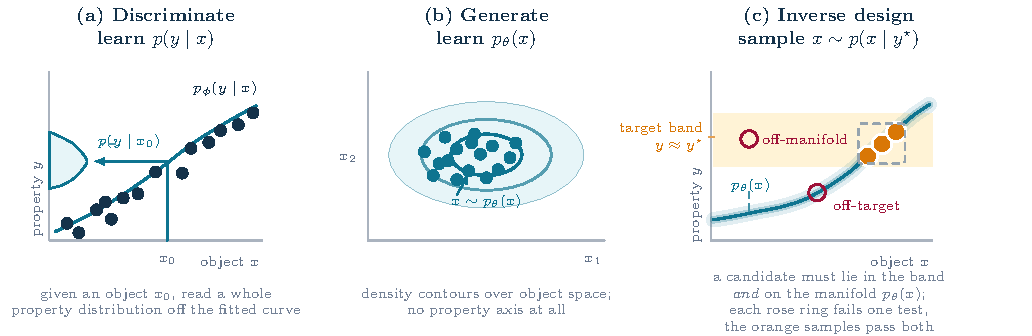
\includegraphics[width=\textwidth]{discriminate_generate_inverse.pdf}
  \vfill
  \begin{concept}{条件概率}
    判别模型学 $p(y\mid x)$：给定对象预测性质。生成模型学 $p(x)$：哪些对象本身合理。逆向设计要的是 $p(x\mid y)$：满足目标性质、又仍然合理的对象。
  \end{concept}
\end{frame}

\begin{frame}{生成模型要提供的两种基本能力}
  \centering
  \begin{tikzpicture}[x=1mm,y=1mm]
    \foreach \i/\t/\f/\a/\b/\c in {%
      0/采样/{$x\sim p_\theta$}/生成新图像、新分子/续写一段文本/为蒙特卡洛提供样本,%
      1/评估密度/{$p_\theta(x)$}/判断一个样本是否合理/异常检测、模型比较/重要性重加权}{%
      \node[draw=GSlate!40,fill=GMist,rounded corners=1.5pt,minimum width=67.8mm,minimum height=28mm,anchor=north west] (b\i) at (\i*72,0) {};
      \node[anchor=north west,font=\bfseries,text=GNavy] at (\i*72+3,-2.5) {\t};
      \node[anchor=north east,text=GTeal] at (\i*72+65,-2.5) {\f};
      \node[anchor=north west,font=\small,text width=60mm,align=left] at (\i*72+3,-11) {\a\\\b\\\c};}
    \node[draw=GTeal!50,fill=GTeal!6,rounded corners=1.5pt,minimum width=139.8mm,minimum height=10mm,anchor=north west,font=\small,text width=133.8mm,align=left] at (0,-31) {\textbf{条件化}：把 $c$ 作为输入，两种能力都有条件版本 $p_\theta(x\mid c)$。\\逆向设计、文生图、按提示词回答都属于这一类。};
  \end{tikzpicture}
  \vfill
  \begin{takeaway}
    很少有模型能同时廉价地做好这两件事：GAN（生成对抗网络）采样快但给不出密度；能量模型的密度写法最灵活，采样却很慢；自回归模型两者兼有，代价是只能逐个生成。第二讲的各类模型就是在这里做不同的取舍。
  \end{takeaway}
\end{frame}

\begin{frame}{想一想：直接优化预测器}
  \begin{columns}[c]
    \begin{column}{0.5\textwidth}
      训练好一个性质预测器 $f_\phi(x)$：输入材料结构 $x$，输出某项性能。它在测试集上误差很小。
      \vspace{3mm}

      逆向设计最直接的做法：从某个 $x$ 出发做梯度上升
      \[
        x\leftarrow x+\eta\,\nabla_xf_\phi(x),
      \]
      一直走到预测性能刷新纪录。
    \end{column}
    \begin{column}{0.46\textwidth}
      \begin{hook}
        这样得到的 $x$，是一个好材料吗？
        \par\medskip
        \opt{A}{是：预测器在测试集上很准}
        \opt{B}{不一定：那它会是什么？}
      \end{hook}
    \end{column}
  \end{columns}
\end{frame}

\begin{frame}{逆向设计：先验乘以似然}
  \begin{columns}[c]
    \begin{column}{0.4\textwidth}
      \[
        p(x\mid y^\star)=\frac{\orange{p_\phi(y^\star\mid x)}\;\teal{p_\theta(x)}}{p(y^\star)}
      \]
    \end{column}
    \begin{column}{0.56\textwidth}
      \small
      \begin{tabularx}{\linewidth}{@{}l X@{}}
        \teal{先验 $p_\theta(x)$} & 生成模型：这个 $x$ 像不像真实数据？\\
        \orange{似然 $p_\phi(y^\star\mid x)$} & 性质预测器：这个 $x$ 达到目标 $y^\star$ 了吗？\\
        分母 $p(y^\star)$ & 与 $x$ 无关，只负责让总概率为 1
      \end{tabularx}
    \end{column}
  \end{columns}
  \vspace{3mm}
  \centering
  \input{figures/bayes_panels.tex}
  \vfill
  \begin{answer}
    多半不是。预测器 $p_\phi$ 只在训练数据附近可靠，只最大化似然，会一路走到数据之外、预测器误判的地方（中图 \rose{$\times$}）。图像上有同样的现象：优化出来的条纹图案，被分类器以 99\% 以上的置信度认作“海星”（Nguyen 等，2015）。乘上先验后，留下的候选既达到目标，又像真实数据。
  \end{answer}
\end{frame}

\begin{frame}{条件分布从哪里来：两条路线}
  \begin{columns}[T]
    \begin{column}{0.61\textwidth}
      \textbf{路线 A：先建模，再用贝叶斯公式拼出来}
      \[
        p(x\mid y)=\frac{\orange{p_\phi(y\mid x)}\,\teal{p_\theta(x)}}{p(y)},\quad
        p(y)=\int \orange{p_\phi(y\mid x)}\,\teal{p_\theta(x)}\,dx
      \]
      \small
      分子对任意 $x$ 都能逐点算；分母 $p(y)$（记作 $Z_y$）要对所有 $x$ 积分，高维时算不出来。绕开分母：
      \begin{itemize}
        \item \textbf{马尔可夫链蒙特卡洛（MCMC）}：只用两个候选的后验之比，分母约掉
        \item \textbf{变分推断}：用可算的 $q$ 逼近后验，分母只贡献常数
      \end{itemize}
    \end{column}
    \begin{column}{0.36\textwidth}
      \textbf{路线 B：直接学习条件分布}
      \[
        \max_\psi\;\E_{(x,y)}\log p_\psi(x\mid y)
      \]
      \small
      \begin{itemize}
        \item $y$ 作为网络输入：文生图里是文字描述，大语言模型里是提示词
        \item 网络结构保证归一化，没有分母要算
      \end{itemize}
    \end{column}
  \end{columns}
  \vfill
  \small
  \begin{tabularx}{\textwidth}{@{}>{\color{GNavy}}l X X@{}}
    \toprule
    & 路线 A：先验 $\times$ 似然 & 路线 B：直接学 $p_\psi(x\mid y)$\\
    \midrule
    需要的数据 & 大量无标签的 $x$，加少量带性质的 $(x,y)$ & 大量配对的 $(x,y)$\\
    换一个目标性质 & 只换预测器 $p_\phi$，先验可复用 & 重新收集配对数据、重新训练\\
    主要代价 & 归一化常数 $Z_y$：推断慢、只能近似 & 配对数据昂贵\\
    \bottomrule
  \end{tabularx}
  \par\vspace{0.5mm}
  {\footnotesize\slate{归一化常数 $Z$ 是贯穿全课的难点，后面每个模型都要说明它怎样处理 $Z$。}}
\end{frame}

% ====================================================================
\section{神经网络：一族可学习的函数}

\begin{frame}{为什么需要神经网络}
  \begin{columns}[c]
    \begin{column}{0.46\textwidth}
      生成模型要表示的都是高维函数：条件概率 $p(y\mid x)$、decoder $p(x\mid z)$、能量 $E(x)$、score $\nabla_x\log p(x)$……
      \begin{itemize}
        \item 高维空间无法查表
        \item 需要一族参数化函数 $f_\theta$：足够灵活，又能用梯度高效地调整参数 $\theta$
        \item 神经网络满足这两点；参数可多达 $10^{9}$--$10^{12}$
      \end{itemize}
    \end{column}
    \begin{column}{0.5\textwidth}
      \centering
      \begin{tikzpicture}[x=1mm,y=1mm]
        \node[nteal,minimum width=20mm] (d) at (0,20) {样本 $(x_i,y_i)$};
        \node[nnavy,minimum width=20mm] (m) at (34,20) {模型 $f_\theta$};
        \node[nsoft,minimum width=20mm] (o) at (34,4) {预测 $f_\theta(x_i)$};
        \node[norange,minimum width=20mm] (l) at (0,4) {损失 $L(\theta)$};
        \node[norange,minimum width=20mm] (g) at (0,-12) {梯度 $\nabla_\theta L$};
        \node[nnavy,minimum width=20mm] (u) at (34,-12) {更新 $\theta$};
        \draw[ar] (d) -- (m);
        \draw[ar] (m) -- (o);
        \draw[ar] (o) -- (l);
        \draw[arorange] (l) -- node[lblo,left] {自动微分} (g);
        \draw[arorange] (g) -- node[lblo,below] {优化器} (u);
        \draw[ar] (u.east) -- ++(6,0) |- (m.east);
      \end{tikzpicture}
      \par\vspace{2mm}
      {\small\slate{训练链：前向得到损失，反向得到梯度，再更新参数}}
    \end{column}
  \end{columns}
\end{frame}

\begin{frame}{回归：拟合一条曲线}
  \begin{columns}[c]
    \begin{column}{0.5\textwidth}
      \begin{tikzpicture}
        \begin{axis}[genai,width=7.4cm,height=5.4cm,xmin=0,xmax=6.5,ymin=-1.6,ymax=1.6,xlabel={$x$},ylabel={$y$},xtick=\empty,ytick=\empty,domain=0:6.5]
          \addplot[name path=up,draw=none] {sin(deg(x))+0.3};
          \addplot[name path=dn,draw=none] {sin(deg(x))-0.3};
          \addplot[GSky] fill between[of=up and dn];
          \addplot[GTeal] {sin(deg(x))};
          \addplot[only marks,mark=*,mark size=1.3pt,GOrange] coordinates {(0.2,0.35)(0.6,0.45)(1.0,0.95)(1.4,0.88)(1.8,1.05)(2.2,0.70)(2.6,0.62)(3.0,0.05)(3.4,-0.15)(3.8,-0.72)(4.2,-0.80)(4.6,-1.05)(5.0,-0.85)(5.4,-0.88)(5.8,-0.30)(6.2,0.02)};
          \node[font=\scriptsize,text=GTeal,anchor=west] at (axis cs:3.9,0.9) {$f_\theta(x)$};
          \node[font=\scriptsize,text=GSlate,anchor=west] at (axis cs:3.9,0.55) {$\pm\sigma$ 噪声带};
        \end{axis}
      \end{tikzpicture}
    \end{column}
    \begin{column}{0.48\textwidth}
      选一个带参数的函数 $f_\theta$，用数据决定参数，最小化均方误差（MSE）：
      \[
        L(\theta)=\frac1N\sum_{i=1}^N\bigl(f_\theta(x_i)-y_i\bigr)^2
      \]
      训练损失小只说明见过的样本拟合得好；泛化要用测试数据检验。
      \vspace{2mm}
      \begin{concept}{高斯似然}
        设 $y=f_\theta(x)+\varepsilon$，$\varepsilon\sim\mathcal N(0,\sigma^2)$，则
        $-\log p(y\mid x)=(y-f_\theta(x))^2/2\sigma^2+\text{常数}$。最小二乘就是这个模型下的极大似然。
      \end{concept}
    \end{column}
  \end{columns}
\end{frame}

\begin{frame}{分类：网络输出一个分布}
  \begin{columns}[c]
    \begin{column}{0.52\textwidth}
      \centering
      \begin{tikzpicture}[x=1mm,y=1mm]
        \foreach \i/\c/\z in {0/猫/2.0,1/狗/0.5,2/鸟/-1.0}{%
          \fill[GSlate!45] (\i*7,12) rectangle ++(5,\z*5);
          \node[font=\scriptsize] at (\i*7+2.5,3) {\c};
          \node[font=\tiny,text=GSlate] at (\i*7+2.5,{\z>0 ? 12+\z*5+2 : 14}) {\z};}
        \draw[GSlate!60] (-1,12) -- (20,12);
        \node[lbl,anchor=north] at (9.5,-1) {logit $z_k$};
        \draw[ar] (22,14) -- node[lbl,above] {softmax} (34,14);
        \foreach \i/\c/\p in {0/猫/0.786,1/狗/0.175,2/鸟/0.039}{%
          \fill[GTeal!80] (36+\i*7,6) rectangle ++(5,\p*30);
          \node[font=\scriptsize] at (36+\i*7+2.5,3) {\c};
          \node[font=\tiny,text=GSlate] at (36+\i*7+2.5,\p*30+8) {\p};}
        \draw[GSlate!60] (35,6) -- (57,6);
        \node[lbl,anchor=north] at (46,-1) {概率 $q_k=e^{z_k}/\sum_j e^{z_j}$};
      \end{tikzpicture}
      \par\vspace{3mm}
      {\small 真实类别为“猫”：交叉熵 $\mathrm{CE}=-\log q_{\text{猫}}=-\log 0.786\approx0.24$}
      \par\vspace{2mm}
      \begin{takeaway}
        网络输出的是一个分布的参数。VAE 的 decoder、语言模型的输出层都沿用这个思路。
      \end{takeaway}
    \end{column}
    \begin{column}{0.46\textwidth}
      \small
      \setlength{\abovedisplayskip}{3pt}\setlength{\belowdisplayskip}{3pt}%
      logit $z=f_\theta(x)$ 是网络最后一层的实数输出。
      \par\vspace{2mm}
      \textbf{二分类}（logistic / sigmoid）
      \[
        q=P(y=1\mid x)=\sigma(z)=\frac{1}{1+e^{-z}}
      \]
      损失：$\ell=-y\log q-(1-y)\log(1-q)$，$y\in\{0,1\}$
      \par\vspace{2mm}
      \textbf{$K$ 分类}（softmax）
      \[
        q_k=P(y=k\mid x)=\frac{e^{z_k}}{\sum_{j=1}^{K}e^{z_j}}
      \]
      损失：$\ell=-\log q_{y}$，只取真实类别那一项
      \par\vspace{2mm}
      {\footnotesize\slate{$\sigma$ 是 $K=2$ 时的 softmax（logit 取 $(z,0)$）。两种损失都叫交叉熵，分别是 Bernoulli 与 categorical 分布的负对数似然。}}
    \end{column}
  \end{columns}
\end{frame}

\begin{frame}{多层感知机}
  \begin{columns}[c]
    \begin{column}{0.5\textwidth}
      \[
        f_\theta(x)=W_2\,\sigma(W_1x+b_1)+b_2
      \]
      \begin{itemize}
        \item 矩阵乘法混合输入的各个分量
        \item 逐元素的非线性激活 $\sigma$ 让函数可以弯曲
        \item 去掉 $\sigma$，多层仿射变换仍是一个仿射变换
        \item 加深网络就是反复组合这两种操作；参数 $\theta=(W_1,b_1,W_2,b_2,\ldots)$ 全部由数据学出
      \end{itemize}
    \end{column}
    \begin{column}{0.48\textwidth}
      \centering
      \begin{tikzpicture}[x=1mm,y=1mm]
        \foreach \i in {0,1,2}{\node[circle,draw=GTeal,fill=GSky,minimum size=5mm,inner sep=0pt] (x\i) at (0,\i*9+4) {\scriptsize $x_{\i}$};}
        \foreach \j in {0,...,4}{\node[circle,draw=GNavy,fill=white,minimum size=5mm,inner sep=0pt] (h\j) at (20,\j*7) {\scriptsize $\sigma$};}
        \node[circle,draw=GOrange,fill=GAmber,minimum size=5mm,inner sep=0pt] (y) at (40,14) {\scriptsize $f$};
        \foreach \i in {0,1,2}{\foreach \j in {0,...,4}{\draw[GSlate!50] (x\i) -- (h\j);}}
        \foreach \j in {0,...,4}{\draw[GSlate!50] (h\j) -- (y);}
        \node[lbl] at (10,-5) {$W_1,b_1$};
        \node[lbl] at (30,-5) {$W_2,b_2$};
      \end{tikzpicture}
      \par\vspace{2mm}
      \begin{tikzpicture}
        \begin{axis}[genai,width=3.6cm,height=2.8cm,xmin=-3,xmax=3,ymin=-0.3,ymax=3,xtick=\empty,ytick=\empty,domain=-3:3,title={\scriptsize ReLU},title style={yshift=-1.5ex}]
          \addplot[GNavy] {max(0,x)};
        \end{axis}
      \end{tikzpicture}\hspace{2mm}
      \begin{tikzpicture}
        \begin{axis}[genai,width=3.6cm,height=2.8cm,xmin=-5,xmax=5,ymin=-0.1,ymax=1.1,xtick=\empty,ytick=\empty,domain=-5:5,title={\scriptsize sigmoid},title style={yshift=-1.5ex}]
          \addplot[GNavy] {1/(1+exp(-x))};
        \end{axis}
      \end{tikzpicture}
    \end{column}
  \end{columns}
\end{frame}

\begin{frame}{隐藏层在做特征变换}
  \centering
  \begin{tikzpicture}[x=1mm,y=1mm]
    \begin{scope}[shift={(22,22)}]
      \draw[GSlate!60] (-20,-20) rectangle (20,20);
      \foreach \a in {0,45,...,315}{\node[dotT] at (\a:5.5) {};}
      \foreach \a in {15,45,...,345}{\node[dotO] at (\a:14) {};}
      \draw[GRose,dashed,line width=0.8pt] (-18,-7) -- (18,9);
      \node[lblr,anchor=north] at (0,-21) {输入空间：没有一条直线能分开};
      \node[lbl] at (-15,17) {$x_1,x_2$};
    \end{scope}
    \draw[ar,line width=1pt] (47,22) -- node[lbl,above] {$h=\sigma(W_1x+b_1)$} (79,22);
    \begin{scope}[shift={(84,2)}]
      \draw[GSlate!60] (0,0) rectangle (40,40);
      \foreach \y [count=\k] in {6,10,14,18,22,26,30,34}{\node[dotT] at ({6+mod(\k,3)*2},\y) {};}
      \foreach \y [count=\k] in {5,8,11,14,17,20,23,26,29,32,35,38}{\node[dotO] at ({28+mod(\k,4)*2.2},\y) {};}
      \draw[GTeal,line width=1pt] (18,2) -- (18,38);
      \node[lblt,anchor=north] at (20,-1) {特征空间（横轴 $h_1\sim\|x\|^2$）：一条直线即可};
    \end{scope}
  \end{tikzpicture}
  \vfill
  \begin{takeaway}
    最后一层只是线性的分类器或回归器；前面各层学到的，是让问题变简单的表示。所需的特征由训练数据和损失共同决定，不需要人工设计。
  \end{takeaway}
\end{frame}

\begin{frame}{梯度下降与随机梯度}
  \begin{columns}[c]
    \begin{column}{0.46\textwidth}
      \centering
      \begin{tikzpicture}[x=1mm,y=1mm]
        \foreach \r in {1,2,3,4,5}{\draw[GSlate!45,rotate=25] (0,0) ellipse ({\r*5.6} and {\r*2.4});}
        \fill[GNavy] (0,0) circle (0.9);
        \draw[GTeal,line width=1pt,-{Latex[length=1.6mm]}] (-24,-4) .. controls (-14,-9) and (-6,-4) .. (-0.8,-0.4);
        \draw[GOrange,line width=0.8pt,-{Latex[length=1.6mm]}] (-24,-4) -- (-21,-11) -- (-18,-3) -- (-14,-9) -- (-12,-2) -- (-8,-7) -- (-6,0) -- (-3,-3.5) -- (-1,0.4);
        \node[lblt,anchor=west] at (-2,-14) {全数据梯度：平滑};
        \node[lblo,anchor=west] at (-2,-18) {小批量梯度：带噪声};
      \end{tikzpicture}
    \end{column}
    \begin{column}{0.52\textwidth}
      \[
        \theta_{k+1}=\theta_k-\eta\,\nabla_\theta L(\theta_k)
      \]
      \begin{itemize}
        \item $\eta$ 是学习率；实际常用 Adam 等自适应优化器
        \item 非凸问题中只保证沿局部下降方向走
      \end{itemize}
      \begin{concept}{蒙特卡洛估计}
        $\nabla L=\frac1N\sum_{i=1}^N\nabla\ell_i$ 是对数据分布求期望；每次随机取 $B$ 个样本，
        $\frac1B\sum_{i\in\mathcal B}\nabla\ell_i$ 是它的无偏估计，方差 $\propto1/B$。这就是随机梯度下降（SGD）。
      \end{concept}
    \end{column}
  \end{columns}
\end{frame}

\begin{frame}{反向传播：沿计算图使用链式法则}
  \centering
  \begin{tikzpicture}[x=1mm,y=1mm]
    \node[nteal] (x) at (0,0) {$x$};
    \node[nnavy] (z) at (26,0) {$z=W_1x+b_1$};
    \node[nnavy] (h) at (56,0) {$h=\sigma(z)$};
    \node[nnavy] (y) at (86,0) {$\hat y=W_2h+b_2$};
    \node[norange] (l) at (116,0) {$\ell(\hat y,y)$};
    \draw[ar] (x) -- (z); \draw[ar] (z) -- (h); \draw[ar] (h) -- (y); \draw[ar] (y) -- (l);
    \node[lbl,anchor=south] at (58,6) {前向：逐层计算，保存中间结果};
    \draw[arorange] (l.south) to[bend left=28] node[lblo,below] {$\delta_{\hat y}=\partial\ell/\partial\hat y$} (y.south);
    \draw[arorange] (y.south) to[bend left=28] node[lblo,below] {$\delta_h=W_2^\top\delta_{\hat y}$} (h.south);
    \draw[arorange] (h.south) to[bend left=28] node[lblo,below] {$\delta_z=\sigma'(z)\odot\delta_h$} (z.south);
    \node[lblo,anchor=north] at (86,-16) {$\partial\ell/\partial W_2=\delta_{\hat y}h^\top$};
    \node[lblo,anchor=north] at (26,-16) {$\partial\ell/\partial W_1=\delta_zx^\top$};
  \end{tikzpicture}
  \vspace{3mm}
  \begin{itemize}
    \item 一次反向传播得到对全部参数的梯度，代价只是前向计算的几倍，与参数个数无关
    \item 自动微分负责算梯度，优化器负责用梯度；两者是训练链中不同的步骤
    \item 计算图中若有“从分布中抽样”这一步，梯度不能直接穿过，需要专门的估计方法（第二讲附录）
  \end{itemize}
\end{frame}

\begin{frame}{表达能力与泛化}
  \centering
  \foreach \t/\f/\c in {欠拟合/{0.15-0.12*x}/GRose,恰当/{sin(deg(x))}/GTeal,过拟合/{sin(deg(x))+0.32*sin(deg(5.2*x))}/GRose}{%
  \begin{tikzpicture}
    \begin{axis}[genai,width=4.6cm,height=3.6cm,xmin=0,xmax=6.5,ymin=-1.6,ymax=1.6,xtick=\empty,ytick=\empty,domain=0:6.5,samples=300,title={\small\t},title style={yshift=-1ex}]
      \addplot[only marks,mark=*,mark size=1pt,GOrange] coordinates {(0.2,0.35)(0.6,0.45)(1.0,0.95)(1.4,0.88)(1.8,1.05)(2.2,0.70)(2.6,0.62)(3.0,0.05)(3.4,-0.15)(3.8,-0.72)(4.2,-0.80)(4.6,-1.05)(5.0,-0.85)(5.4,-0.88)(5.8,-0.30)(6.2,0.02)};
      \addplot[\c] {\f};
    \end{axis}
  \end{tikzpicture}}
  \vspace{2mm}
  \begin{columns}[T]
    \begin{column}{0.5\textwidth}
      \small
      \textbf{通用近似定理}：单隐藏层网络只要足够宽，就能在紧集上把任意连续函数逼近到任意精度。这是存在性结论：它不保证网络小、数据够、梯度下降能找到参数，也不保证训练区域外的预测正确。
    \end{column}
    \begin{column}{0.47\textwidth}
      \begin{concept}{偏差与方差}
        误差来自三处：函数族不够灵活（近似误差），优化没找到好参数（优化误差），有限样本导致过拟合（估计误差）。
      \end{concept}
    \end{column}
  \end{columns}
\end{frame}

\begin{frame}{小结：一条训练链}
  \begin{takeaway}[本节要点]
    \begin{enumerate}
      \item 损失函数就是在某个选定分布下的负对数似然：MSE 对应高斯，交叉熵对应 categorical
      \item 训练就是用小批量样本估计期望梯度，再沿梯度迭代
      \item 神经网络是一族灵活、可求梯度的函数，它的输出常常是一个分布的参数
    \end{enumerate}
  \end{takeaway}
  \vspace{4mm}
  到这里，网络拟合的还是一个数或一个条件分布 $p(y\mid x)$。生成模型要拟合的是整个高维分布 $p(x)$，而我们只有它的样本。
  \vspace{2mm}
  \begin{center}
    \navy{接下来的问题：怎样衡量两个分布的差距？}
  \end{center}
\end{frame}

% ====================================================================
\section{怎样比较两个分布}

\begin{frame}{从拟合一个数到拟合一个分布}
  我们有 $p_{\mathrm{data}}$ 的样本和模型 $p_\theta$，需要一个“距离” $D(p_{\mathrm{data}},p_\theta)$：只用样本就能估计；$D=0$ 当且仅当两分布相同；对 $\theta$ 可求梯度。
  \vspace{2mm}

  \small
  \begin{tabularx}{\textwidth}{@{}l X X@{}}
    \toprule
    散度 & 直观含义 & 在哪里出现\\
    \midrule
    $\KL(p_{\mathrm{data}}\Vert p_\theta)$ & 数据在模型下的平均对数似然 & 自回归、Flow；VAE 与扩散优化它的上界\\
    $\KL(q\Vert\pi)$ & 模型样本在目标下是否合理 & 变分推断、统计物理、RLHF\\
    $\mathrm{JSD}(p\Vert q)$ & Jensen--Shannon 散度 $\tfrac12\KL(p\Vert m)+\tfrac12\KL(q\Vert m)$，$m=\tfrac12(p+q)$：分类器能否分辨两组样本 & GAN\\
    Fisher 散度 & $\tfrac12\E_p\|\nabla_x\log p-\nabla_x\log q\|^2$：两者的 score 是否处处一致 & score matching、扩散\\
    \bottomrule
  \end{tabularx}
  \vspace{3mm}
  \begin{takeaway}
    选择哪一种散度，就是选择哪一类误差被重视；不同生成模型的行为差异很多来自这里。
  \end{takeaway}
\end{frame}

\begin{frame}{KL 散度（相对熵）}
  \begin{columns}[T]
    \begin{column}{0.52\textwidth}
      \[
        \KL(p\Vert q)=\E_{x\sim p}\!\left[\log\frac{p(x)}{q(x)}\right]
      \]
      \begin{itemize}
        \item $\KL\geq0$，等号当且仅当 $p=q$
        \item 不对称：$\KL(p\Vert q)\neq\KL(q\Vert p)$，期望取在哪个分布下，哪里的误差就被重视
        \item 信息论含义：用为 $q$ 设计的编码去编码来自 $p$ 的样本，平均多付出的信息量
      \end{itemize}
    \end{column}
    \begin{column}{0.45\textwidth}
      \begin{keystep}[非负性]
        由 Jensen 不等式（$\log$ 是凹函数）：
        \keyeq{-\KL(p\Vert q)&=\E_p\log\frac{q}{p}\\&\leq\log\E_p\frac{q}{p}=\log\!\int q=0}
      \end{keystep}
      \begin{concept}{相对熵}
        KL 是两个分布的对数似然比在 $p$ 下的期望；假设检验中它决定了区分 $p$ 与 $q$ 的错误率衰减速度。
      \end{concept}
    \end{column}
  \end{columns}
\end{frame}

\begin{frame}{极大似然就是最小化前向 KL}
  \begin{itemize}
    \item 数据集 $\{x^{(i)}\}_{i=1}^N$ 给出经验分布 $\hat\pi$，每个样本权重 $1/N$
    \item 模型族 $p_\theta$：训练要在其中找一个离 $\hat\pi$ 最近的分布
  \end{itemize}
  \begin{keystep}
    \keyeq{
      \KL(\hat\pi\Vert p_\theta)
      &=\E_{\hat\pi}[\log\hat\pi(x)]-\E_{\hat\pi}[\log p_\theta(x)]
      =\underbrace{\text{常数}}_{\text{与 }\theta\text{ 无关}}
      -\frac1N\sum_{i=1}^N\log p_\theta(x^{(i)})}
  \end{keystep}
  \begin{columns}[T]
    \begin{column}{0.5\textwidth}
      \begin{concept}{极大似然估计（MLE）}
        在模型族里找离经验分布最近的分布；前面的 MSE 与交叉熵都是它的特例。
      \end{concept}
    \end{column}
    \begin{column}{0.47\textwidth}
      \small
      用这个目标训练只需要两样东西：
      \begin{itemize}
        \item 数据样本
        \item 能逐点计算 $\log p_\theta(x)$
      \end{itemize}
      第二条正是“显式密度”模型必须满足的要求。
    \end{column}
  \end{columns}
\end{frame}

\begin{frame}{想一想：一个高斯拟合两个峰}
  \begin{columns}[c]
    \begin{column}{0.55\textwidth}
      \begin{tikzpicture}
        \begin{axis}[genai,width=8.4cm,height=5.4cm,
          xmin=-5,xmax=5,ymin=0,ymax=0.72,ytick=\empty,xtick=\empty,
          xlabel={$x$},samples=241,domain=-5:5]
          \addplot[fill=GSlate!18,draw=GSlate!70]
            {0.5*exp(-(x+2)^2/(2*0.36))/(0.6*sqrt(2*pi))+0.5*exp(-(x-2)^2/(2*0.36))/(0.6*sqrt(2*pi))}
            \closedcycle;
          \addplot[GTeal]{exp(-x^2/(2*4.36))/(2.088*sqrt(2*pi))};
          \addplot[GOrange,dashed]{exp(-(x-2)^2/(2*0.36))/(0.6*sqrt(2*pi))};
          \node[font=\small\bfseries,text=GTeal] at (axis cs:0,0.25) {A};
          \node[font=\small\bfseries,text=GOrange] at (axis cs:2.75,0.6) {B};
          \node[font=\scriptsize,text=GSlate] at (axis cs:-2,0.43) {目标 $p$};
        \end{axis}
      \end{tikzpicture}
    \end{column}
    \begin{column}{0.42\textwidth}
      目标 $p$ 有两个峰，模型 $q$ 却只能是一个高斯。
      \vspace{3mm}
      \begin{hook}
        哪一个 $q$ 离 $p$ 更近？
        \par\medskip
        \opt{A}{横跨两峰的宽高斯}
        \opt{B}{只盖住一个峰的窄高斯}
      \end{hook}
    \end{column}
  \end{columns}
\end{frame}

\begin{frame}{两个方向，两种行为}
  \begin{columns}[T]
    \begin{column}{0.55\textwidth}
      \begin{tikzpicture}
        \begin{axis}[genai,width=8.4cm,height=5.4cm,
          xmin=-5,xmax=5,ymin=0,ymax=0.72,ytick=\empty,xtick=\empty,
          xlabel={$x$},samples=241,domain=-5:5,
          legend style={at={(0.02,0.98)},anchor=north west}]
          \addplot[fill=GSlate!18,draw=GSlate!70]
            {0.5*exp(-(x+2)^2/(2*0.36))/(0.6*sqrt(2*pi))+0.5*exp(-(x-2)^2/(2*0.36))/(0.6*sqrt(2*pi))}
            \closedcycle;
          \addlegendentry{目标 $p$}
          \addplot[GTeal]{exp(-x^2/(2*4.36))/(2.088*sqrt(2*pi))};
          \addlegendentry{$\min_q\KL(p\Vert q)$}
          \addplot[GOrange,dashed]{exp(-(x-2)^2/(2*0.36))/(0.6*sqrt(2*pi))};
          \addlegendentry{$\min_q\KL(q\Vert p)$}
        \end{axis}
      \end{tikzpicture}
    \end{column}
    \begin{column}{0.43\textwidth}
      \small
      用单个高斯 $q$ 拟合双峰目标 $p$：
      \begin{itemize}
        \item \teal{前向 KL} 在 $p$ 下取期望：$p$ 有质量而 $q\approx0$ 处代价极大，$q$ 只好横跨两峰
        \item \orange{反向 KL} 在 $q$ 下取期望：$q$ 只需留在 $p$ 的高概率区，于是落在一个峰上
      \end{itemize}
      \begin{answer}
        A、B 各是一个方向的最优解，“更近”取决于期望取在哪个分布下。A 覆盖所有模式，峰值却落在 $p$ 几乎没有概率的地方；B 的样本都像真的，却丢掉一个模式。第二讲比较 VAE、GAN 时会再用到这张图。
      \end{answer}
    \end{column}
  \end{columns}
\end{frame}

\begin{frame}{玻尔兹曼分布}
  \begin{columns}[T]
    \begin{column}{0.48\textwidth}
      统计物理中，温度 $T$ 下构型 $x$ 的概率为
      \[
        \pi(x)=\frac{e^{-E(x)/k_BT}}{Z},\quad Z=\int e^{-E(x)/k_BT}dx
      \]
      \begin{itemize}
        \item $E(x)$：能量，越低越可能
        \item $T$：温度。$T\to0$ 时集中到能量最低处；$T$ 很高时趋于均匀
        \item $Z$：配分函数，对所有构型求和或积分
      \end{itemize}
      \vspace{1mm}
      \begin{caution}[难点]$Z$ 算不出来，密度只知道到一个常数因子；采样只能用 MCMC 这类只依赖概率比值的方法。\end{caution}
    \end{column}
    \begin{column}{0.5\textwidth}
      \begin{tikzpicture}
        \begin{axis}[genai,width=7.0cm,height=5.6cm,
          xmin=-2,xmax=2,ymin=0,ymax=1.15,ytick=\empty,xtick={-1,1},
          xlabel={$x$},samples=161,domain=-2:2,
          legend style={at={(0.5,1.02)},anchor=south,legend columns=3}]
          \addplot[GSlate!60,dotted] {0.35*(x^2-1)^2};
          \addlegendentry{$E(x)$}
          \addplot[GOrange]{exp(-(x^2-1)^2/1.5)};
          \addlegendentry{$T$ 高}
          \addplot[GTeal]{exp(-(x^2-1)^2/0.08)};
          \addlegendentry{$T$ 低}
        \end{axis}
      \end{tikzpicture}
      \par{\scriptsize\slate{双势阱能量与两个温度下的未归一化密度 $e^{-E/k_BT}$}}
    \end{column}
  \end{columns}
\end{frame}

\begin{frame}{玻尔兹曼分布从哪里来}
  \begin{columns}[T]
    \begin{column}{0.53\textwidth}
      \begin{keystep}[最大熵推导]
        只知道平均能量 $\sum_xp(x)E(x)=U$ 时，求熵最大的分布：
        \keyeq{\max_p\;&-\sum_xp\log p-\alpha\Bigl(\sum_xp-1\Bigr)\\&-\beta\Bigl(\sum_xpE-U\Bigr)}
        对 $p(x)$ 求导令其为零：$-\log p-1-\alpha-\beta E(x)=0$，
        \keyeq{p(x)=\frac{e^{-\beta E(x)}}{Z},\qquad \beta=\frac{1}{k_BT}}
      \end{keystep}
      \begin{concept}{最大熵原理}
        在给定约束下最不额外假设的分布；$\beta$ 是平均能量约束的拉格朗日乘子。
      \end{concept}
    \end{column}
    \begin{column}{0.44\textwidth}
      \small
      \textbf{例：Ising 模型}\quad $s_i=\pm1$，
      \[E(s)=-J\textstyle\sum_{\langle ij\rangle}s_is_j\]
      \centering
      \begin{tikzpicture}[x=1mm,y=1mm]
        \foreach \r in {0,...,5}{\foreach \c in {0,...,5}{%
          \pgfmathtruncatemacro{\flip}{(\r==2 && \c==4) || (\r==4 && \c==1)}
          \ifnum\flip=1 \fill[GOrange] (\c*3.4,\r*3.4) rectangle ++(3,3);\else\fill[GTeal] (\c*3.4,\r*3.4) rectangle ++(3,3);\fi}}
        \foreach \r in {0,...,5}{\foreach \c in {0,...,5}{%
          \pgfmathtruncatemacro{\s}{mod(\r*7+\c*5+\r*\c*3,4)}
          \ifnum\s<2 \fill[GTeal] (\c*3.4+26,\r*3.4) rectangle ++(3,3);\else\fill[GOrange] (\c*3.4+26,\r*3.4) rectangle ++(3,3);\fi}}
        \node[lbl,anchor=north] at (10,-1) {低温：有序};
        \node[lbl,anchor=north] at (36,-1) {高温：无序};
      \end{tikzpicture}
      \par\vspace{2mm}\raggedright
      $N=100$ 个自旋就有 $2^{100}\approx10^{30}$ 个构型，$Z$ 无法逐项求和。
    \end{column}
  \end{columns}
\end{frame}

\begin{frame}{反向 KL 就是变分自由能}
  目标是玻尔兹曼分布 $\pi=e^{-\beta E}/Z$，用一个可采样、可算密度的分布 $q$ 去逼近它：
  \begin{keystep}
    \keyeq{
      \KL(q\Vert\pi)&=\E_q[\log q]+\beta\,\E_q[E]+\log Z
      =\beta\bigl(F[q]-F\bigr)\geq0,\\[1mm]
      F[q]&=\underbrace{\E_q[E]}_{\text{平均能量}}-T\underbrace{S[q]}_{-k_B\E_q[\log q]},\qquad F=-k_BT\log Z}
  \end{keystep}
  \begin{columns}[T]
    \begin{column}{0.5\textwidth}
      \begin{itemize}
        \item 最小化反向 KL 等价于最小化变分自由能 $F[q]$，下界 $F$ 在 $q=\pi$ 时取到
        \item 需要从 $q$ 采样，并能逐点算出 $E(x)$ 与 $\log q(x)$（熵项要用）；不需要 $Z$，也不需要数据
      \end{itemize}
    \end{column}
    \begin{column}{0.47\textwidth}
      \begin{concept}{变分原理}
        能量项把 $q$ 推向低能构型，熵项阻止 $q$ 塌缩到一点；平衡就是低能与高熵的折中。
      \end{concept}
    \end{column}
  \end{columns}
\end{frame}

\begin{frame}{两种学习情形}
  \centering
  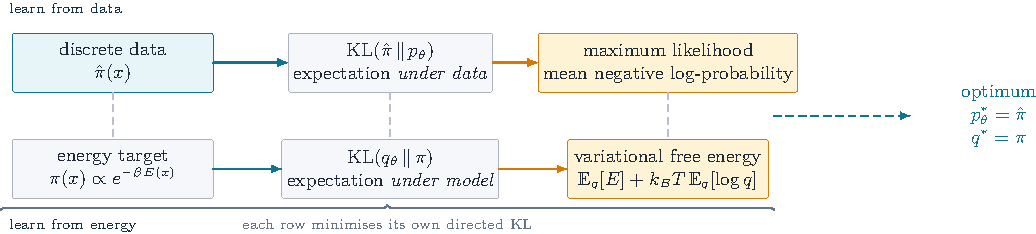
\includegraphics[width=0.94\textwidth]{mle_free_energy.pdf}
  \vspace{2mm}
  \small
  \begin{tabularx}{\textwidth}{@{}l l l X@{}}
    \toprule
    手中有什么 & 目标 & 期望在谁下 & 典型问题\\
    \midrule
    数据样本 $\hat\pi$ & $\KL(\hat\pi\Vert p_\theta)$：极大似然 & 数据 & 生成模型训练（第二、三讲）\\
    能量函数 $E(x)$ & $\KL(q\Vert\pi)$：变分自由能 & 模型 & 统计物理采样、变分推断、RLHF（基于人类反馈的强化学习，第三讲）\\
    \bottomrule
  \end{tabularx}
\end{frame}

\begin{frame}{归一化常数：反复出现的难点}
  \begin{columns}[T]
    \begin{column}{0.44\textwidth}
      同一个积分以不同面目出现：
      \begin{itemize}
        \item 贝叶斯后验中的 $Z_y$
        \item 玻尔兹曼分布中的 $Z$
        \item 任何写成 $p_\theta=\tilde p_\theta/Z_\theta$ 的模型
      \end{itemize}
      \vspace{2mm}
      高维积分难算，也让采样变难：不知道 $Z$，就没法像查分布表那样直接抽出独立样本，只能用 MCMC 这类只依赖概率比值的方法，代价是链要混合、样本彼此相关。
    \end{column}
    \begin{column}{0.53\textwidth}
      \small
      \begin{tabularx}{\linewidth}{@{}>{\color{GNavy}}l X@{}}
        \toprule
        处理方式 & 对应模型\\
        \midrule
        构造上自动归一化 & 自回归、Flow\\
        优化一个下界 & VAE\\
        不需要密度 & GAN\\
        只用密度比值 & 能量模型 + MCMC\\
        只用 $\nabla_x\log p$ & score matching、扩散\\
        \bottomrule
      \end{tabularx}
      \vspace{2mm}
      \begin{takeaway}
        各类生成模型的一个主要区别，就是怎样对付 $Z$。
      \end{takeaway}
    \end{column}
  \end{columns}
\end{frame}

% ====================================================================
\section{生成模型地图}

\begin{frame}{想一想：随机涂像素}
  \begin{columns}[c]
    \begin{column}{0.42\textwidth}
      \centering
      \begin{tikzpicture}[x=1mm,y=1mm]
        \pgfmathsetseed{7}
        \foreach \i in {0,...,23}{\foreach \j in {0,...,23}{%
          \pgfmathsetmacro{\r}{rnd}\pgfmathsetmacro{\g}{rnd}\pgfmathsetmacro{\b}{rnd}%
          \definecolor{px}{rgb}{\r,\g,\b}%
          \fill[px] (\i*2,\j*2) rectangle ++(2,2);}}
        \draw[GSlate!60] (0,0) rectangle (48,48);
        \node[lbl,anchor=north] at (24,-1.5) {随机抽出的一张“图”};
      \end{tikzpicture}
    \end{column}
    \begin{column}{0.54\textwidth}
      一张 $256\times256$ 的彩色图，每个像素的 R、G、B 各从 $0$--$255$ 中随机取值。
      \vspace{3mm}
      \begin{hook}
        平均要抽多少次，才能抽到一张看起来像照片的图？
        \par\medskip
        \opt{A}{约 $10^{10}$ 次}
        \opt{B}{约 $10^{100}$ 次}
        \opt{C}{宇宙寿命内也抽不到}
      \end{hook}
    \end{column}
  \end{columns}
\end{frame}

\begin{frame}{高维分布难在哪里}
  \begin{answer}
    C。可能的图共有 $256^{3\times256\times256}=256^{196608}\approx10^{473000}$ 张，而宇宙中的原子约 $10^{80}$ 个。真实照片只占其中极薄的一层（右图浅蓝带），随机抽样几乎永远落在它外面。
  \end{answer}
  \vspace{1mm}
  \begin{columns}[c]
    \begin{column}{0.5\textwidth}
      \begin{itemize}
        \item \textbf{维度灾难}：每维分 $M$ 格，直方图需要 $M^d$ 个格子。$M=10$、$d=100$ 时是 $10^{100}$
        \item \textbf{集中在低维结构}：真实图像只占像素空间中极小的一部分，随机像素几乎从不像一张照片
        \item \textbf{只有有限样本}：要从 $N$ 个点推断整个分布，还要能生成没见过的样本
      \end{itemize}
      \vspace{2mm}
      于是需要三样东西：灵活的函数族（神经网络）、只依赖样本的训练目标（如极大似然）、可执行的采样程序。
    \end{column}
    \begin{column}{0.46\textwidth}
      \centering
      \begin{tikzpicture}[x=1mm,y=1mm]
        \pgfmathsetseed{5}
        \fill[GMist] (0,0) rectangle (50,40);
        \foreach \j in {1,...,70}{\fill[GSlate!45] (25+25*rand,20+20*rand) circle (0.5);}
        \draw[GSky,line width=7mm,line cap=round] plot[smooth] coordinates {(6,8) (16,26) (28,18) (40,32) (46,22)};
        \foreach \x/\y in {6.5/9,8.5/13,10.5/17.5,12.5/21.5,15/25,17.5/26,20/24.5,23/21.5,26/19,28.5/18.5,31/20.5,33.5/23.5,36/27.5,38.5/30.5,41/31,43.5/28,45.5/23}{%
          \node[dotT,minimum size=1.3mm] at (\x,\y) {};}
        \node[lblt,anchor=south] at (25,41) {数据：一条弯曲的薄带};
        \node[lbl,anchor=north] at (25,-1) {灰点：随机抽取的“像素组合”};
      \end{tikzpicture}
    \end{column}
  \end{columns}
\end{frame}

\begin{frame}{六条路线}
  \centering
  \input{figures/genmap.tex}
  \vfill
  {\small 上一行能算出（或界住）$p(x)$，下一行绕开归一化；底部是每条路线借用的概率工具。}
\end{frame}

\begin{frame}{第一讲小结}
  \begin{takeaway}[带走的几件事]
    \begin{enumerate}
      \item 生成模型学的是整个分布 $p(x)$ 或 $p(x\mid c)$；两种基本能力是采样与密度评估，条件生成是它们的条件版本
      \item 神经网络是一族可求梯度的函数，常输出分布的参数；常见损失都是某个分布的负对数似然
      \item 极大似然等价于最小化前向 KL；从能量出发的变分自由能等价于最小化反向 KL
      \item 两个方向的 KL 行为不同：前向覆盖模式，反向抓住模式
      \item 归一化常数 $Z$ 是高维概率建模的核心难点，各类模型的区别就在怎样处理它
    \end{enumerate}
  \end{takeaway}
  \vspace{3mm}
  \navy{下一讲}：沿地图依次看自回归、Flow、VAE、GAN 与能量模型怎样处理 $p(x)$。
\end{frame}

\end{document}
